\documentclass[10pt,twocolumn]{article}
\usepackage[utf8]{inputenc}
\usepackage[T1]{fontenc}
\usepackage{mathptmx}
\usepackage[letterpaper,top=0.75in,bottom=0.85in,left=0.7in,right=0.7in,columnsep=0.24in]{geometry}
\usepackage{graphicx,booktabs,amsmath,siunitx,xcolor,tikz,array,cite,url,lettrine}
\usepackage[font=footnotesize,labelfont=bf,labelsep=period,skip=4pt]{caption}
\usepackage{titlesec,fancyhdr}
\usetikzlibrary{arrows.meta,positioning,calc}
\sisetup{detect-all,range-phrase=--,per-mode=symbol,separate-uncertainty=true}
\setcounter{secnumdepth}{0}
\titleformat{\section}{\normalfont\large\bfseries\color{black!80}}{}{0pt}{}
\titlespacing*{\section}{0pt}{9pt plus 2pt}{3pt}
\renewcommand{\figurename}{Figure}
\renewcommand{\tablename}{Table}
\captionsetup[table]{position=top}
\pagestyle{fancy}\fancyhf{}
\fancyhead[L]{\footnotesize\itshape IEEE Design \& Test --- Special Issue: SBCCI 2026}
\fancyhead[R]{\footnotesize\itshape Alencar et al.: Burn-In Thermal Control Sets What Aging Sensors Can See}
\fancyfoot[C]{\footnotesize\thepage}
\renewcommand{\headrulewidth}{0.3pt}
\setlength{\parskip}{0pt}
\definecolor{pid}{HTML}{1F5FBF}\definecolor{bb}{HTML}{D9661F}
\newcommand{\Tmin}{T_{\min}}
\newcommand{\tint}{\tau_{\mathrm{int}}}
\hyphenation{Arrhe-nius}
\begin{document}

\twocolumn[{%
\begin{center}
{\footnotesize\scshape Feature Article --- Special Issue: SBCCI 2026}\\[6pt]
{\LARGE\bfseries Burn-In Thermal Control Sets What\\[2pt] Aging Sensors Can See}\\[8pt]
{\normalsize Danilo Alencar, Alisson Barros, Arthur Pamplona, Andre Grangeiro, Lucas Nogueira, and Jarbas Silveira}\\
{\small\itshape Universidade Federal do Cear\'a, Fortaleza, Brazil}\\[3pt]
{\normalsize Fabian Vargas}\\
{\small\itshape IHP -- Leibniz Institute for High Performance Microelectronics, Frankfurt (Oder), Germany}\\[8pt]
\begin{minipage}{0.86\textwidth}
\small\noindent\textbf{\textit{Abstract}---}On-chip aging sensors validated under burn-in increasingly feed silicon lifecycle management (SLM), yet burn-in standards constrain the chamber, not the die the sensor sees. Using one FPGA, one slack sensor, and two thermal-control architectures, we show that bench architecture sets both the stress delivered and the time needed to see aging. A thermostatic oven under-delivers Arrhenius acceleration by 1.65$\times$ almost entirely through mean die-temperature shortfall, not ripple. A 212.6-hour PID campaign resolves aging after 34 hours; a thermostatic bench would need about 55. We propose a five-item reporting checklist for sensor-instrumented burn-in.\\[4pt]
\noindent\textbf{\textit{Keywords}---}Burn-in, on-chip aging sensor, silicon lifecycle management, FPGA, thermal control, acceleration factor, detectability.
\end{minipage}
\end{center}
\vspace{6pt}}]
\renewcommand{\thefootnote}{}\footnotetext{\scriptsize This article extends ``Quantifying the Effect of Burn-In Thermal Control on Delivered Acceleration Factor and On-Chip Slack-Sensor Fidelity in an FPGA Target,'' presented at the 39th Symposium on Integrated Circuits and Systems Design (SBCCI 2026)~\cite{sbcci26}. Digital Object Identifier to be assigned.}\renewcommand{\thefootnote}{\arabic{footnote}}



% ---------------------------------------------------------------
\section{Introduction}
\lettrine[lines=2,findent=1pt,nindent=0pt]{O}{n-chip} aging sensors are moving from research prototypes into the silicon lifecycle management (SLM) stack, where their readings drive adaptive voltage scaling (AVS), remaining-useful-life (RUL) estimation, and maintenance decisions~\cite{kashyap,niemann}. Before a sensor is trusted in the field, it is usually validated under accelerated burn-in: the device is heated and over-volted, and the sensor is expected to report the resulting delay degradation. Validation of FPGA aging sensors against standardized burn-in has a decade-long history~\cite{valdes}, and a recent survey maps the broader landscape of aging detection on embedded hardware~\cite{lanzieri}.

The standards that govern burn-in, JEDEC JESD22-A108~\cite{jedec} and MIL-STD-883 Method~1015~\cite{mil}, specify the \emph{chamber}: ambient temperature, its tolerance, and the applied bias. A powered digital device under test (DUT), however, heats itself, and an on-chip sensor samples the \emph{die}. Between the two sits the bench's thermal-control loop. Bidmeshki~\textit{et al.}\ showed in simulation that digital sensors raise false aging alarms when process, voltage, and temperature (PVT) are not corrected~\cite{bidmeshki}; the bench is the dominant source of exactly that PVT variation during validation.

Our SBCCI~2026 paper~\cite{sbcci26} compared a thermostatic (bang-bang) oven and a closed-loop PID oven on the same FPGA and sensor and found that the two benches delivered different stress and different reversible noise. That result left a practical question open, which this article answers: \emph{how long must a burn-in run last before a sensor can see aging at all, and how much does the bench change that time?} The answer requires knowing both the aging rate the bench induces and the noise it injects, which a 23-hour campaign cannot provide.

Fig.~\ref{fig:chain} summarizes the argument. Beyond the conference version, the main contributions of this work are:
\begin{enumerate}\setlength{\itemsep}{1pt}\setlength{\parsep}{0pt}
\item \textbf{A source decomposition of the delivered-stress bias.} We show that the 1.65$\times$ acceleration-factor gap between benches is set by the mean die-temperature shortfall, while thermostat ripple contributes about 1\%, and we translate it into a die-level tracking budget.
\item \textbf{A 212.6-hour sustained-stress campaign}, first reported here, in which the on-chip sensor resolves a permanent slack drift of $-18.3$\,m\,cnt/h after PVT correction.
\item \textbf{A detectability bound for sensor-instrumented burn-in.} From the Cram\'er--Rao bound we derive the minimum burn-in duration needed to see aging (34 hours on the PID bench), explaining why 23-hour campaigns cannot resolve it.
\item \textbf{A projection of the bench penalty on detectability.} Combining the measured noise and stress ratios, a thermostatic bench needs about 1.6$\times$ longer to see aging, and a 24-hour aging alarm loses a third of its reliability.
\item \textbf{The construction and validation of the PID bench}, including model identification, tuning sensitivity, and an independent architecture comparison at a second setpoint.
\item \textbf{A five-item reporting checklist} that reliability and SLM teams can apply to any 1-Hz burn-in log.
\end{enumerate}

\begin{figure*}[!t]
\centering
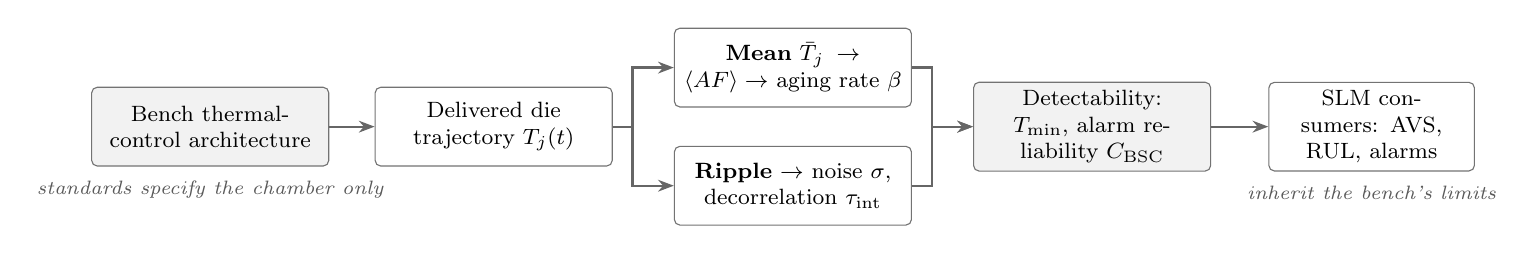
\begin{tikzpicture}[
  box/.style={draw=black!55,rounded corners=2pt,align=center,font=\footnotesize,inner sep=3pt,text width=28mm,minimum height=10mm,fill=white},
  hl/.style={box,fill=black!5},
  arr/.style={-{Stealth[length=2mm]},thick,black!60},
  lab/.style={font=\scriptsize\itshape,text=black!65}]
\node[hl] (bench) at (0,0) {Bench thermal-control architecture};
\node[box] (die) at (3.6,0) {Delivered die trajectory $T_j(t)$};
\node[box] (mean) at (7.4,0.75) {\textbf{Mean} $\bar T_j \rightarrow \langle AF\rangle \rightarrow$ aging rate $\beta$};
\node[box] (rip) at (7.4,-0.75) {\textbf{Ripple} $\rightarrow$ noise $\sigma$, decorrelation $\tint$};
\node[hl] (det) at (11.2,0) {Detectability: $\Tmin$, alarm reliability $C_{\mathrm{BSC}}$};
\node[box,text width=24mm] (slm) at (14.75,0) {SLM consumers: AVS, RUL, alarms};
\draw[arr] (bench) -- (die);
\draw[arr] (die.east) -- ++(2.5mm,0) |- (mean.west);
\draw[arr] (die.east) -- ++(2.5mm,0) |- (rip.west);
\draw[arr] (mean.east) -- ++(2.5mm,0) |- (det.west);
\draw[arr] (rip.east) -- ++(2.5mm,0) |- (det.west);
\draw[arr] (det) -- (slm);
\node[lab,below=0.6mm of bench] {standards specify the chamber only};
\node[lab,below=0.6mm of slm] {inherit the bench's limits};
\end{tikzpicture}
\caption{The argument of this article. The bench sets the die-temperature trajectory; its mean fixes the stress delivered and therefore the aging signal, its ripple sets the reversible noise. Signal and noise together fix how long a burn-in must run before a sensor can detect aging, and that limit propagates into every SLM function trained on the result.}
\label{fig:chain}
\end{figure*}

% ---------------------------------------------------------------
\section{Instrument, Benches, and Evidence Base}

\textbf{Sensor and DUT.} The DUT is a 28\,nm Xilinx Artix-7 FPGA on a Nexys~4~DDR board. The instrument is our auto-tuning slack sensor~\cite{sbcci25}: an MMCM dynamic phase shift advances a sampling clock in \SI{19.85}{ps} steps until an XOR comparator detects that the monitored path's output has not yet settled, and the number of steps is reported as the path's slack in counts (cnt). The sensor recalibrates autonomously, so it tracks slack without manual retuning~\cite{sbcci25}. Die temperature and core voltage $V_{\mathrm{CCINT}}$ come from the on-chip XADC. Because the same XADC is used throughout, its absolute offset cancels in the within-run statistics reported here. A programmable supply sets the core voltage, and a supervisory PC logs slack, die temperature, voltage, oven temperature and supply current, time-aligned at \SI{1}{Hz}.

\textbf{Two benches.} Both use the same 30-liter laboratory drying oven. The \emph{bang-bang} bench keeps the oven's stock thermostat, the arrangement typical of academic aging labs. A rate-limited software loop (\SI{5}{mV} steps, at least \SI{2}{s} apart) holds the mean supply voltage; its bandwidth is far below the thermostat cycle, so it corrects the mean but not the cycle. The \emph{PID} bench replaces the thermostat with a microcontroller driving a zero-crossing solid-state relay in a \SI{5}{s} time-proportioning window. An open-loop step at 50\% power identified a first-order-plus-dead-time model with gain \SI{1.56}{\celsius} per percent, dead time \SI{150.6}{s}, and time constant \SI{1307.2}{s}. Skogestad's SIMC rules~\cite{simc} gave the initial gains. Empirical refinement then lowered the integral gain and added a derivative term ($K_p=2.78$, $K_i=\SI{1.06e-3}{\per\s}$, $K_d=\SI{5.0}{s}$), and a soft-start ramp limits thermal shock at power-up. The whole stack uses commodity parts: a Cortex-M0+ board, an NTC thermistor in a ratiometric divider, an SSR, and a SCPI-controlled supply.

\textbf{Is the PID a fair baseline?} A natural objection is that a carefully tuned PID is being compared with a poorly tuned thermostat. Two facts answer it. First, the thermostatic oven is not a strawman: it is the unmodified commercial chamber. Second, tuning matters even within PID: at a \SI{100}{\celsius} setpoint, the textbook SIMC gains gave \SI{1.33}{\celsius} steady-state standard deviation and \SI{5.2}{\celsius} overshoot, against \SI{0.40}{\celsius} and no overshoot after refinement. The bench is a design choice at every level, which is the point of this article.

\textbf{Evidence base.} Table~\ref{tab:evidence} lists the four campaigns used. The two 23.08-hour runs share every commanded parameter (\SI{80}{\celsius} oven air, \SI{1.3}{V}, \SI{115}{\celsius} intended die temperature) and differ only in the thermal loop~\cite{sbcci26}. The 212.6-hour PID run, first reported here, was acquired on the same device during its second week of burn-in, after a first week at \SI{115}{\celsius}; it held \SI{93.9 \pm 1.8}{\celsius} oven air, \SI{1.400}{V} on-die, and a \SI{125.1 \pm 1.8}{\celsius} die. It logged 768,884 samples after soak with no manual sensor recalibration. A one-hour \SI{100}{\celsius} comparison of the oven air under each controller provides an independent check of the architecture effect at a second setpoint. Every run discards its first hour as thermal soak.

\begin{table}[!t]
\centering
\caption{Evidence base. All campaigns use the same oven; all sensor runs use the same Artix-7 device and slack sensor.}
\label{tab:evidence}
\footnotesize
\setlength{\tabcolsep}{3pt}
\begin{tabular}{@{}l l l l@{}}
\toprule
Campaign & Bench & Conditions & Used here for \\
\midrule
23.08\,h pair~\cite{sbcci26} & BB vs.\ PID & 80\,\textdegree C air, 1.3\,V & Stress, noise ratios \\
212.6\,h run & PID & 125\,\textdegree C die, 1.4\,V & Aging rate, $\sigma$, $\tint$ \\
1\,h, 100\,\textdegree C & BB vs.\ PID & oven air only & Second setpoint \\
1\,h, 100\,\textdegree C & SIMC vs.\ tuned & oven air only & Tuning sensitivity \\
\bottomrule
\end{tabular}
\end{table}

% ---------------------------------------------------------------
\section{Delivered Stress: The Mean, Not the Ripple}

Burn-in accelerates bias-temperature instability and related mechanisms according to the Arrhenius relation, and for a time-varying die temperature the stress actually delivered is the trajectory average
\begin{equation}
\langle AF\rangle=\Big\langle \exp\!\Big[\frac{E_a}{k_B}\Big(\frac{1}{T_{\mathrm{use}}}-\frac{1}{T_j(t)}\Big)\Big]\Big\rangle_t .
\label{eq:af}
\end{equation}
Under identical commands, the thermostatic bench held the die at \SI{107.73}{\celsius} on average and the PID bench at \SI{117.04}{\celsius}, a \SI{9.31}{\celsius} gap. At $E_a=\SI{0.7}{eV}$ and $T_{\mathrm{use}}=\SI{55}{\celsius}$ this gives $\langle AF\rangle=31.1$ and 51.3, a 1.65$\times$ ratio, or \SI{718}{h} versus \SI{1184}{h} of equivalent use-condition stress over the same wall-clock time~\cite{sbcci26}. The thermostat itself reached its \SI{80}{\celsius} air setpoint within its hysteresis window. The shortfall arises because, during each off phase, the self-heated die sheds heat into cooling air, whereas under PID the air stays at setpoint and the die's self-heating offset rides fully on top of it.

A common intuition is that thermostat ripple is what distorts the stress, since the exponential in Eq.~\eqref{eq:af} weights hot excursions more than cold ones. The data contradict this. Modeling each run's die temperature as normally distributed with its measured mean and standard deviation (\SI{2.64}{\celsius} bang-bang, \SI{1.25}{\celsius} PID) reproduces the reported $\langle AF\rangle$ to within 0.1. In that model, ripple raises the thermostatic bench's AF by only 1.0\% and the PID bench's by 0.2\%. Fig.~\ref{fig:stress}(a) separates the two effects across activation energies: the mean shortfall alone predicts the full bias, and ripple slightly \emph{offsets} it. The bias is 1.43--1.90$\times$ over $E_a\in[0.5,0.9]$\,eV, so its direction does not depend on the mechanism assumed.

The practical consequence is that a lab cannot repair the thermostatic bench by tightening hysteresis; it must know the die's mean temperature, which requires die-level telemetry. A first-order expansion of Eq.~\eqref{eq:af} gives the mean die-temperature error $\delta$ that keeps the delivered AF within a fraction $\eta$ of nominal,
\begin{equation}
\delta\approx\frac{k_B T_{\mathrm{set}}^2}{E_a}\,\ln(1+\eta),
\label{eq:delta}
\end{equation}
with $T_{\mathrm{set}}$ in kelvin. At \SI{115}{\celsius} and \SI{0.7}{eV}, a $\pm$5\%, $\pm$10\%, or $\pm$20\% AF tolerance allows only 0.91, 1.77, or \SI{3.38}{\celsius}. Fig.~\ref{fig:stress}(b) places both benches on this budget: the bang-bang shortfall of \SI{7.27}{\celsius} exceeds even the 20\% budget by more than twofold, while the PID bench overshot its die target by \SI{2.04}{\celsius}, within a 12\% budget. The PID bench is not error-free, but its error is small, stable, and visible.

\begin{figure*}[!t]
\centering
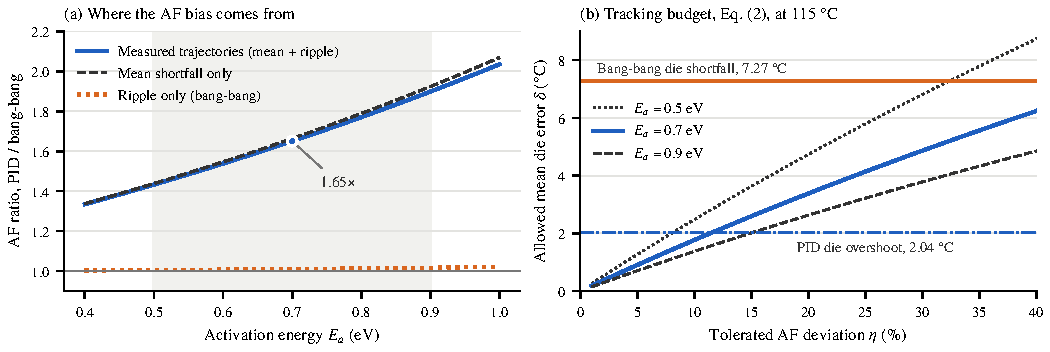
\includegraphics[width=\textwidth]{fig_stress.pdf}
\caption{Delivered stress in the 23.08-hour pair. (a) PID-to-bang-bang ratio of delivered acceleration factor versus activation energy. The bias is reproduced by the mean die-temperature shortfall alone; ripple contributes about 1\% (shaded: commonly assumed $E_a$ range). (b) Allowed mean die-temperature error from Eq.~\eqref{eq:delta} versus tolerated AF deviation, with each bench's measured mean die error.}
\label{fig:stress}
\end{figure*}

The architecture effect is not specific to one setpoint. At \SI{100}{\celsius}, the oven air under the stock thermostat had a \SI{3.29}{\celsius} standard deviation, \SI{9.0}{\celsius} peak-to-peak swing, and \SI{7.2}{\celsius} maximum error, against \SI{0.40}{\celsius}, \SI{2.1}{\celsius}, and \SI{1.8}{\celsius} under PID. These are chamber-air figures, and they are exactly what the standards assess. The die-level data above show what they leave out: the thermostatic chamber's air ripple was the visible symptom, but its mean die shortfall was the consequential error.

% ---------------------------------------------------------------
\section{Reversible Noise: What the Bench Writes Into the Sensor}

The slack a sensor reports mixes a slow, permanent aging term with a fast, reversible PVT term. In the 23.08-hour pair, die temperature and voltage linearly explain 92.1\% of slack variance under bang-bang and 59.2\% under PID. A lower $R^2$ under PID is not lower fidelity: the controlled bench simply injects less environmental variance to explain. The decisive figure is the residual after joint temperature--voltage regression, \SI{0.904}{cnt} (bang-bang) versus \SI{0.726}{cnt} (PID), a 25\% larger noise floor for any AVS or alarm calibrated on the thermostatic bench~\cite{sbcci26}. The supply also oscillated more under bang-bang (\SI{6.1}{mV} versus \SI{3.6}{mV} standard deviation) despite active compensation, because the die's leakage follows the thermal cycle.

$R^2$ has two limits as a bench-quality metric: it sees only linear dependence, and it has no transferable unit. Mutual information $I(S;T,V)$ between slack and environment addresses both. On the 212.6-hour PID run, the environment carries 1.132\,bits about the slack (95\% block-bootstrap interval 1.091--1.176), against a surrogate null of 0.097\,bits and a slack entropy of 3.43\,bits. A linear PVT correction removes 93\% of the reversible information (0.656 to 0.046\,bits on detrended signals) and leaves a residual of \SI{0.84}{cnt}, consistent with the 23-hour PID value. We also tested whether the coupling is nonlinear beyond what $R^2$ captures. The apparent excess of mutual information over the linear equivalent does not survive detrending, so we attribute it to shared slow drift rather than instantaneous nonlinearity, and a linear correction suffices at a single operating point. We therefore recommend mutual information as a reporting unit, not as evidence about the underlying physics.

% ---------------------------------------------------------------
\begin{figure*}[!t]
\centering
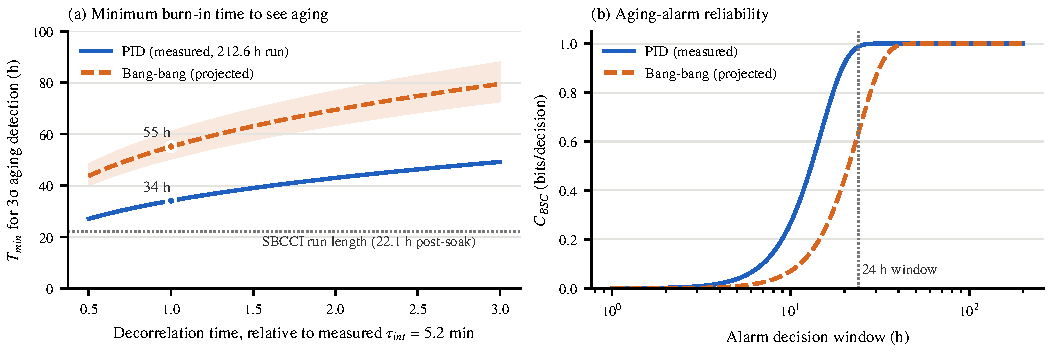
\includegraphics[width=\textwidth]{fig_detect.pdf}
\caption{Detectability on the 212.6-hour PID run and its projection to a thermostatic bench using the ratios measured in the 23.08-hour pair. (a) Minimum burn-in duration for 3$\sigma$ detection, Eq.~\eqref{eq:tmin}, versus decorrelation time (band: $E_a$ from 0.5 to 0.9\,eV). (b) Capacity of a threshold aging alarm, modeled as a binary symmetric channel, versus decision window.}
\label{fig:detect}
\end{figure*}

\section{Detectability: When Can a Sensor See Aging?}

\textbf{Aging is resolved.} After PVT correction, the 212.6-hour residual drifts at \SI{-18.3}{m\,cnt/h}. A Bayesian fit on decorrelated samples gives \SI{-18.2}{m\,cnt/h} with a 95\% credible interval of $[-19.2,-17.2]$, and the correlation of slack with time strengthens from $-0.35$ before correction to $-0.73$ after it. The total drift over the run is about \SI{3.9}{cnt}, or \SI{77}{ps} of lost slack. It is small, but it is unambiguous only because the run was long.

\textbf{The minimum burn-in time.} The 1-Hz samples are strongly correlated: the integrated autocorrelation time is $\tint=\SI{314}{s}$, so the 768,884 samples carry only $n_{\mathrm{eff}}=n/2\tint\approx1{,}224$ independent observations. For a least-squares slope over duration $T$, the Cram\'er--Rao bound gives $\mathrm{Var}(\hat\beta)\ge24\,\sigma^2\tint/T^3$. Requiring a drift $\beta$ to exceed three standard errors yields the minimum observation time
\begin{equation}
\Tmin=\left(\frac{216\,\sigma^2\,\tint}{\beta^2}\right)^{1/3}.
\label{eq:tmin}
\end{equation}
With the measured $\sigma=\SI{0.84}{cnt}$ and $\beta=\SI{18.3}{m\,cnt/h}$, $\Tmin=\SI{34}{h}$ (credible interval 33--\SI{36}{h}), and the 3$\sigma$ floor over the full run is \SI{1.2}{m\,cnt/h}, 15$\times$ below the measured rate. This explains a limitation of the conference study: its 23-hour runs, 22.1 hours after soak, were too short by construction to separate aging from bench noise.

\textbf{Projecting to a thermostatic bench.} Eq.~\eqref{eq:tmin} shows how the bench enters: through the noise $\sigma$ and decorrelation time $\tint$ it injects, and through the stress it delivers, which sets $\beta$. The 23.08-hour pair measured both channels on the same device: a thermostatic bench raises the residual by 1.25$\times$ and lowers the delivered AF by 1.65$\times$. If aging rate scales with delivered AF, these two penalties compound. The noise penalty alone lengthens $\Tmin$ by $1.25^{2/3}=1.16\times$, the stress penalty by $1.65^{2/3}=1.40\times$, together 1.62$\times$. Transferred to the long-run operating point, a thermostatic bench would need about \SI{55}{h} instead of \SI{34}{h} (\SIrange{50}{61}{h} over $E_a\in[0.5,0.9]$\,eV). This is a projection from measured ratios, not a second long campaign. It also assumes equal $\tint$, which is optimistic: thermostat cycles add slow correlated structure, and doubling $\tint$ would raise the penalty to about 2.05$\times$ [Fig.~\ref{fig:detect}(a)].



\textbf{Alarm reliability.} SLM functions consume decisions, not slopes. We model a threshold aging alarm that compares windows of length $w$ as a binary symmetric channel with crossover probability $p=Q(\mathrm{SNR}_w/2)$, where $\mathrm{SNR}_w=\beta w/(\sigma\sqrt{2\tint/w})$, and report its capacity $C_{\mathrm{BSC}}=1-H_2(p)$. On the PID run, an hourly alarm is a coin flip ($C\approx0$), while a 24-hour window gives $C=0.99$\,bits per decision [Fig.~\ref{fig:detect}(b)]. Under the projected thermostatic noise and stress, the same 24-hour alarm drops to 0.64\,bits and needs about 39 hours to reach 0.99. A team that chooses its alarm window on one bench and deploys a sensor validated on another will mis-set it.

\textbf{From detectability to failure.} Detectability alone does not say how far the circuit is from failing. Our sensor work validated a flip-flop failure catcher at the end of the monitored path: when slack is driven toward zero by lowering the supply, the catcher records a real timing violation at the sensor-reported failure point, within clock-jitter margin~\cite{sbcci25}. Sensor slack thus has a physical zero, and a detected drift becomes a distance-to-failure under stress. We do not extrapolate a lifetime from one device and one operating point, because bias-temperature aging is sublinear in time; circuit-level failure prediction~\cite{agarwal} needs the operating-point models a single campaign cannot supply. The anchor, however, turns Eq.~\eqref{eq:tmin} from a statistical statement into one an SLM controller can act on.

% ---------------------------------------------------------------
\section{What Labs Should Report}

The standards behave as designed: they bound the chamber, and the thermostatic bench's air ripple would be flagged by them. What they do not bound is the stress and noise reaching a powered die, which is precisely what a critical-path sensor samples. For sensor-instrumented burn-in we propose the five-item report of Table~\ref{tab:checklist}. Each item is computable from a standard 1-Hz log, and together they let a reader judge whether a published aging curve reflects the device or the bench. The two items most often missing in the FPGA aging literature, die-level mean temperature and $\Tmin$, are also the two that change the conclusions most in our data.

\begin{table}[!t]
\centering
\caption{Proposed reporting checklist for sensor-instrumented burn-in, with values from this study.}
\label{tab:checklist}
\footnotesize
\setlength{\tabcolsep}{2.5pt}
\begin{tabular}{@{}p{27mm} p{56mm}@{}}
\toprule
Item & This study \\
\midrule
1. Die trajectory: mean, std.\ dev., error vs.\ target & BB 107.73\,\textdegree C, 2.64, $-$7.27; PID 117.04\,\textdegree C, 1.25, +2.04 \\
2. Delivered $\langle AF\rangle$ with $E_a$ range & BB 31.1, PID 51.3 at 0.7\,eV; ratio 1.43--1.90 \\
3. Post-PVT residual $\sigma$ (and $I(S;T,V)$) & BB 0.904, PID 0.726\,cnt; 1.132\,bits (212.6\,h) \\
4. Decorrelation $\tint$ and $n_{\mathrm{eff}}$ & 314\,s; 1,224 of 768,884 samples \\
5. $\Tmin$ vs.\ run length & 34\,h (PID, measured); $\approx$55\,h (BB, projected) \\
\bottomrule
\end{tabular}
\end{table}

\textbf{Limitations.} All sensor data come from one 28\,nm device, so bench effects are established within-device and not as population statistics. The thermostatic detectability figures are projections that transfer ratios measured at \SI{115}{\celsius}/\SI{1.3}{V} to the \SI{125}{\celsius}/\SI{1.4}{V} long run, and they assume aging rate proportional to delivered AF. A matched-duration thermostatic campaign, a second technology node, and multi-device replication are the natural next steps, and our group is pursuing them on a 16\,nm FinFET platform. There, published drifts are below 0.1\% over 1,000 hours even at elevated stress~\cite{sobas}, so the bench-set detection floor will matter even more than it does at 28\,nm. Statements about JEDEC and MIL-STD conditions are interpretive and do not claim formal chamber certification.

% ---------------------------------------------------------------
\section{Conclusion}

On one FPGA with one sensor, swapping only the oven's thermal loop changed the stress delivered by 1.65$\times$, the sensor's noise floor by 25\%, and the time needed to see aging by roughly 1.6$\times$. The dominant error is the mean die temperature, which chamber-level specifications cannot reveal, not the ripple they police. Sensor-validated burn-in is now an input to SLM, so the bench belongs in the measurement chain, and it should be reported with the same care as the sensor.

% ---------------------------------------------------------------
\renewcommand{\refname}{References}\begin{thebibliography}{12}
\footnotesize
\bibitem{kashyap} R.~Kashyap, ``Silicon lifecycle management (SLM) with in-chip monitoring,'' in \emph{Proc. IEEE Int. Rel. Phys. Symp. (IRPS)}, 2021, pp.~1--6.
\bibitem{niemann} C.~Niemann, M.~Ali, O.~U.~Shah, J.~Heller, and D.~Timmermann, ``Sensor based adaptive voltage scaling on FPGAs: Calibration and parametrization,'' \emph{Integration}, vol.~75, pp.~30--39, 2020.
\bibitem{valdes} M.~Vald\'es-Pe\~na \emph{et al.}, ``Design and validation of configurable online aging sensors in nanometer-scale FPGAs,'' \emph{IEEE Trans. Nanotechnol.}, vol.~12, no.~4, pp.~508--517, 2013.
\bibitem{jedec} JEDEC, \emph{JESD22-A108G: Temperature, Bias, and Operating Life}, 2022.
\bibitem{mil} U.S. Department of Defense, \emph{MIL-STD-883, Method 1015: Burn-In Test}, 2016.
\bibitem{lanzieri} L.~Lanzieri, G.~Martino, G.~Fey, H.~Schlarb, T.~C.~Schmidt, and M.~W\"ahlisch, ``A review of techniques for ageing detection and monitoring on embedded systems,'' \emph{ACM Comput. Surv.}, vol.~57, no.~1, 2024.
\bibitem{bidmeshki} M.-M.~Bidmeshki, G.~Di~Natale, and P.~Maurine, ``On the effect of aging on digital sensors,'' in \emph{Proc. IEEE HOST}, 2020.
\bibitem{sbcci26} D.~Alencar \emph{et al.}, ``Quantifying the effect of burn-in thermal control on delivered acceleration factor and on-chip slack-sensor fidelity in an FPGA target,'' in \emph{Proc. 39th SBCCI}, 2026.
\bibitem{sbcci25} L.~Nogueira \emph{et al.}, ``Auto-tuning aging sensor validated under burn-in, temperature, and voltage variations,'' in \emph{Proc. 38th SBCCI}, 2025, pp.~1--5.
\bibitem{agarwal} M.~Agarwal, B.~C.~Paul, M.~Zhang, and S.~Mitra, ``Circuit failure prediction and its application to transistor aging,'' in \emph{Proc. 25th IEEE VLSI Test Symp. (VTS)}, 2007, pp.~277--286.
\bibitem{simc} S.~Skogestad, ``Simple analytic rules for model reduction and PID controller tuning,'' \emph{J. Process Control}, vol.~13, no.~4, pp.~291--309, 2003.
\bibitem{sobas} J.~Sobas, T.-B.~Airimitoaie, and F.~Marc, ``Development of a high accuracy and stability test bench for ageing measurement of 16\,nm FinFETs based FPGA,'' \emph{Microelectron. Rel.}, vol.~138, 2022.
\end{thebibliography}

% ---------------------------------------------------------------
\section*{Author Biographies}
\footnotesize
\noindent\textbf{Danilo Alencar} is a master's student in Teleinformatics Engineering at the Universidade Federal do Cear\'a (UFC), Fortaleza, Brazil, where he received his B.Sc.\ in computer engineering in 2026, and a researcher at the Laboratory of Electronic Systems and Circuits (LESC). His research interests include RISC-V soft-core architecture, FPGA reliability, aging instrumentation, and silicon lifecycle management. Contact him at danilo.alencar@lesc.ufc.br.

\smallskip\noindent\textbf{Alisson Barros}, \textbf{Arthur Pamplona}, and \textbf{Andre Grangeiro} are with LESC, UFC, Fortaleza, Brazil. Their research interests include FPGA test platforms and reliability instrumentation.

\smallskip\noindent\textbf{Lucas Nogueira} is with LESC, UFC, Fortaleza, Brazil. His research interests include on-chip aging sensors and FPGA delay monitoring. Contact him at lucas.nogueira@lesc.ufc.br.

\smallskip\noindent\textbf{Jarbas Silveira} is a professor at UFC, Fortaleza, Brazil, and leads research at LESC. His research interests include integrated-circuit design, test, and reliability. Contact him at jarbas@lesc.ufc.br.

\smallskip\noindent\textbf{Fabian Vargas} is with IHP -- Leibniz Institute for High Performance Microelectronics, Frankfurt (Oder), Germany. His research interests include on-chip sensors, design for reliability, and silicon lifecycle management. Contact him at vargas@ihp-microelectronics.com.

\end{document}
